%!TEX root = ../thesis.tex
%*******************************************************************************
%                                   Context                                    %
%*******************************************************************************

\chapter{Project Context}

%******************************** Section 1.1 *********************************%
\section{Introduction}
  The aim of this chapter is to contextualize the project by giving its background,
  to present the host company and to define in a later section the main problem as well
  as the way we adresse it.

%******************************** Section 1.2 *********************************%
\section{Project Background}
  This project is about desining and implementing a positive energy worker.
  In addition to powering iExec's infrustructure, this worker serves at the same
  time as a usefull IoT device. It is achieved in the context of the preparation of
  the end of studies project submitted to obtain computer science engineering degree.

%******************************** Section 1.3 *********************************%
\section{Host company}

  \begin{figure}[!h]\centering
    
\includegraphics[width=.5\columnwidth]{2.0-Context/figs/iExec-logo.pdf}
    \caption{iExec's logo}
    % \label{iExec's logo}
  \end{figure}

  Started in 2016, iExec was co-founded by Dr. Gilles Fedak and Pr. Haiwu He.

  Ph.D, CEO and Co-Founder, Dr. Gilles Fedak has been a permanent INRIA research scientist since
  2004 at the ENS in Lyon, France. His research interests lie in Parallel and Distributed
  Computing, with a particular emphasis on the problematic of using large and loosely-coupled
  distributed computing infrastructures to support highly demanding computational and
  data-intensive science. He co-authored about 80 peer-reviewed scientific papers and won two
  Best Paper awards. Pr. Haiwu He, Ph.D, Co-Founder and Head of Asian-Pacific Region was a
  research engineer expert at INRIA Rhone-Alpesin Lyon, France from 2008 to 2014. He has
  published about 30 refereed journal and conference papers. His research interest covers
  peer-to-peer distributed systems, cloud computing, and big data.

  iExec aims at providing decentralized applications running on the blockchain a scalable,
  secure and easy access to the services, data-sets and computing resources they need. This
  technology relies on Ethereum smart contracts and allows the building of a virtual cloud
  infrastructure that provides high-performance computing services on demand.

  iExec leverages a set of research technologies that have been developed at the INRIA and CNRS
  research institutes in the field of Desktop Grid computing. The idea of Desktop Grid
  (aka. Volunteer Computing) is to collect the computer resources that are underutilized on the
  Internet to execute very large parallel applications at the fraction of the cost of a
  traditional supercomputer. iExec relies on XtremWeb-HEP, a mature, solid, and open-source Desktop
  Grid software which implements all the needed features: fault-tolerance, multi-applications,
  multi-users, hybrid public/private infrastructure, deployment of virtual images, data management,
  security and accountability, and many more.

  iExec is developing a new Proof-of-Contribution (PoCo) protocol, that will allow off-chain
  consensus. Thanks to the Proof-of-Contribution, external resource providers will have the usage
  of their resources certified directly in the blockchain.

  iExec aims to deploy a scalable, high-performance, secure and manageable infrastructure sidechain
  that will promote a new form of distributed governance, involving key HPC, big data and cloud
  industry leaders.

  iExec is using its ERC20-compliant token to provide standard and secure payments. RLC which stands for
  "Run on Lots of Computers", can be securely and easily stored, transferred, traded, divided and used
  to make payments. This widely adopted cryptocurrency (87 million RLC are currently in circulation)
  is used to access all iExec's services.

  From a research project, iExec is now a company, whose headquarters are in Lyon, France, with a
  subsidiary in Hong Kong.

%******************************** Section 1.4 *********************************%
\section{Problematic}
  With the huge increase of human dependency on Information Technology for even daily activities,
  comes the massive consumption of electricity. In 2016, global data centers used roughly 416
  terawatts (more than 90 billion kilowatt-hours for just U.S. data centers) or about 3\% of the
  total electricity in terms of percentage, which is nearly 40\% more than the entire United Kingdom.
  Predictions have show that this consumption will double every four years.
  % source: https://www.forbes.com/sites/forbestechcouncil/2017/12/15/
  % why-energy-is-a-big-and-rapidly-growing-problem-for-data-centers/#682a483c5a30
  % 24/08/2018 11:00

  As the “internet of everything” brings innovations such as driverless cars and smart watches,
  the vast network of data centers that have sprung up in the past decade will spread. Moreover,
  the explosion of processing-power demanding technologies like artificial intelligence and
  blockchain is just adding fuel to the fire. For instance, in Japan, studies have shown that
  its data centers would consume its entire electricity supply by 2030 if growth continues at
  today's rate.

  On top of that, internet-connected devices is changing the entire landscape because IoT is
  projected to exceed 20 billion devices by 2020. Given there are currently 10 billion devices,
  doubling that will require massive increases to our data center infrastructure, which will
  massively increase our electricity consumption.

  % It's time that disruptive innovation on the compute side comes to market soon, giving us faster
  % compute engines and architectures that deliver more computational density per watt.

  We are currently stuck with architectures developed some 40 years ago that are not going to
  satisfy humanity’s insatiable thirst for a lot more processing, much faster processing and
  much more energy-efficient processing.

  - embrace fog computing
  - use IoT devices in the right way
  - totally green

  Trend to Fog/Edge computing

  \begin{figure}[!h]\centering
    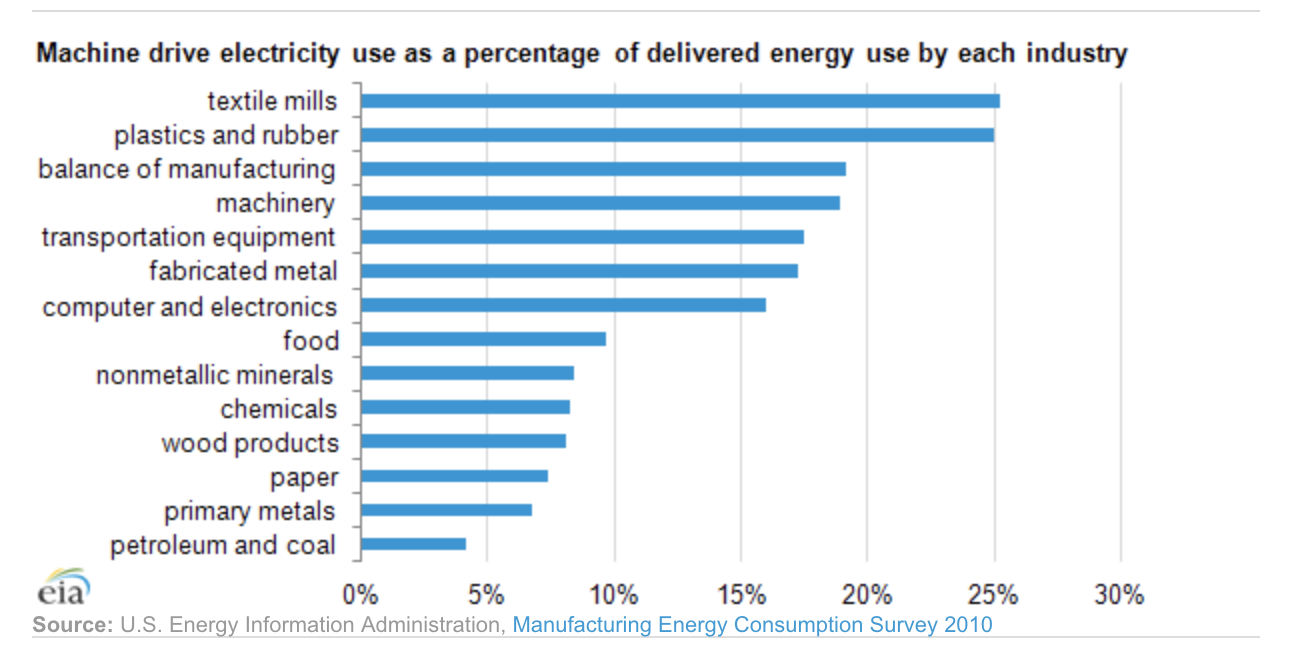
\includegraphics[width=.8\columnwidth]{2.0-Context/figs/Energy-consumption-graph.png}
    \caption{Energy consumption}
    \label{Energy-consumption-graph}
  \end{figure}

  % - Enegy Consumption \\
  % - Idle IoT devices \\
  % - Idle Computing resources 

%******************************** Section 1.5 *********************************%
\section{Suggested Solution}
  - Positive Energy Worker
  - Usefull use cases
  - Multi-functionality IoT devices

%******************************** Section 1.6 *********************************%
\section{Adopted Methodology}
  - To Do

\clearpage